\documentclass[compress, red, 14pt]{beamer}

\usepackage[italian]{babel}
\usepackage[utf8]{inputenc}
\usepackage{kmath,kerkis}
\usepackage[T1]{fontenc}
\usepackage{color}

\usefonttheme{serif}
\usefonttheme{structurebold}

\usebackgroundtemplate{
\includegraphics[width=\paperwidth]{images/background.png}}
\setbeamertemplate{navigation symbols}{}
\definecolor{purple}{RGB}{147,10,0}
\setbeamercolor{structure}{fg=purple}

\setbeamertemplate{items}[circle]
\setbeamercolor*{item}{fg=black}

\newcommand{\highlight}[1]{{\color{purple} \emph{#1}}}

\title{ Extreme \\ Project Evaluation }

\author{
	Jacopo Franzoi \\
	{\scriptsize jacopo.franzoi@gmail.com }
}

\date{
	Italian Agile Day \\
	Milano, 24 Novembre 2012
}

\begin{document}
	\begin{frame}
		\titlepage
	\end{frame}

	\begin{frame}{Introduzione}
		\begin{quote}
			{\small "<{How can you plan a project if you only have a week? [..] You don't have enough time to write a complete set of stories [..] You don't have time to write prototypes so you can estimate the stories from experience}">}
		\end{quote}
		\hfill {\scriptsize K.Beck, Extreme Programming Explained, 1st Edition}

		\begin{itemize}
			\item Diversi Obiettivi
			\begin{itemize}
				\item Indicazioni di budget / effort
				\item Offerta commerciale
			\end{itemize}
		\end{itemize}
	\end{frame}


	\begin{frame}{Una Possibile Strategia}
		\begin{itemize}
			\item Planning in eXtreme Programming (XP)
			\begin{itemize}
				\item \highlight{Strategia}: Esplorazione, Commitment, Steering
				\item \highlight{Valori}: Feedback, Semplicità, Comunicazione
			\end{itemize}

			\item Valutazione Progetti: Steering?
			\begin{itemize}
				\item Granularità grossa
				\item Reporting, Feedback, Kick-Off
			\end{itemize}

		\end{itemize}
	\end{frame}


	\begin{frame}{Esplorazione: Brainstorming}
		\begin{itemize}
			\item Guida il cliente
			\begin{itemize}
				\item Discussione
				\item Presentazioni, documentazione
				\item Siti web esistenti
			\end{itemize}
		\end{itemize}	

		\begin{itemize}
			\item \textbf{Mappa Mentale}
		\end{itemize}

	\end{frame}

	\begin{frame}{Esplorazione: Cosa?}
		\begin{itemize}
			\item Storie / Temi
			\item Scadenze, Eventi importanti
		\end{itemize}

		\begin{itemize}
			\item \textbf{Piano di Rilascio}
			\item \textbf{Modello del Dominio}
		\end{itemize}
	\end{frame}

	\begin{frame}{Esplorazione: Come?}
		\begin{itemize}
			\item \textbf{Architettura Logica}
			\begin{itemize}
				\item Alto Livello
				\item Fattibilità
			\end{itemize}
			\item Hosting
			\begin{itemize}
				\item In-house, Cloud
			\end{itemize}
			\item Spikes
		\end{itemize}

	\end{frame}

	\begin{frame}{Commitment: Stima}
		\begin{itemize}
			\item Complessità
			\item Incertezza
		\end{itemize}

		\begin{itemize}
			\item \textbf{Effort}
		\end{itemize}
	\end{frame}

	\begin{frame}{Commitment: Piano di Rilascio}
		\begin{itemize}
			\item Composizione team
		\end{itemize}

		\begin{itemize}
			\item \textbf{Elapsed}
		\end{itemize}
	\end{frame}
	
	\begin{frame}{Commitment: Economics}
		\begin{itemize}
			\item Sviluppo
			\item Hosting
			\item Servizi
		\end{itemize}

	\end{frame}
	
	\begin{frame}{Reporting}
		\begin{itemize}
			\item Introduzione
			\item Valutazione
			\begin{itemize}
				\item Modello del Dominio, Piano di Rilascio
				\item Tabelle riassuntive: Effort, Elapsed
			\end{itemize}
			\item Soluzione Tecnica
			\begin{itemize}
				\item Architettura Logica, Hosting
			\end{itemize}
			\item Economics
			\begin{itemize}
				\item Tabella riassuntiva: Costi
				\item Non un contratto!
			\end{itemize}
		\end{itemize}
	\end{frame}
	
	\begin{frame}{Sì, ma...}
		\begin{itemize}
			\item Ok per progetti di clienti, ma per prodotti?
			\item Chi paga per questa valutazione?
			\item E dopo? Il contratto? E il kick-off?
		\end{itemize}
		\begin{center}
			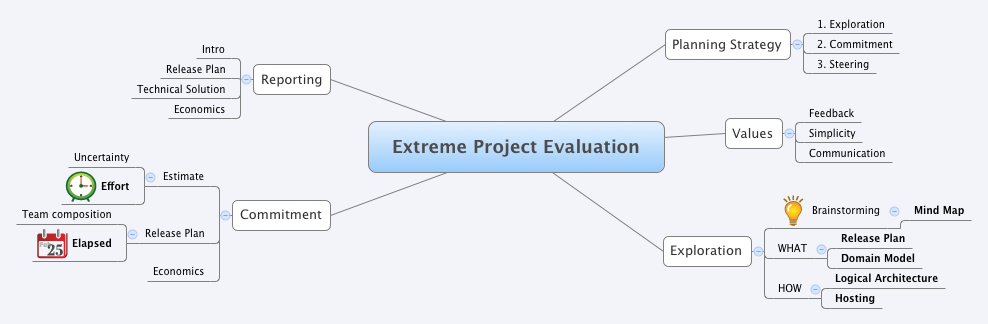
\includegraphics[scale=0.28]{images/takeaway.png}
		\end{center}
	\end{frame}
	
	\begin{frame}{Per Approfondire}
		\begin{itemize}
			\item {\small K.Beck, Extreme Programming Explained, 1st ed.}
			\begin{itemize}
				\item Strategia di Pianificazione
				\item Valori
			\end{itemize}
			\item {\small M.Cohn, Agile Estimating and Planning}
			\begin{itemize}
				\item Incertezza nelle stime
			\end{itemize}
			\item Mind Mapping
			\item Reporting
			\begin{itemize}
				\item LaTeX
				\item Version Control Systems
			\end{itemize}
		\end{itemize}
	\end{frame}

\end{document}